\documentclass{article}

\usepackage{graphicx}
\usepackage{tikz}
\usepackage{tikzsymbols}
\usetikzlibrary{calc,patterns,shapes.geometric}
\pagestyle{empty}
\usepackage[margin=0pt]{geometry}
\geometry{papersize={14in,12in}}

\def\centerarc[#1](#2)(#3:#4:#5){\draw[#1] ($(#2)+({#5*cos(#3)},{#5*sin(#3)})$) arc (#3:#4:#5);}

\begin{document}
	\begin{figure}
		\centering
		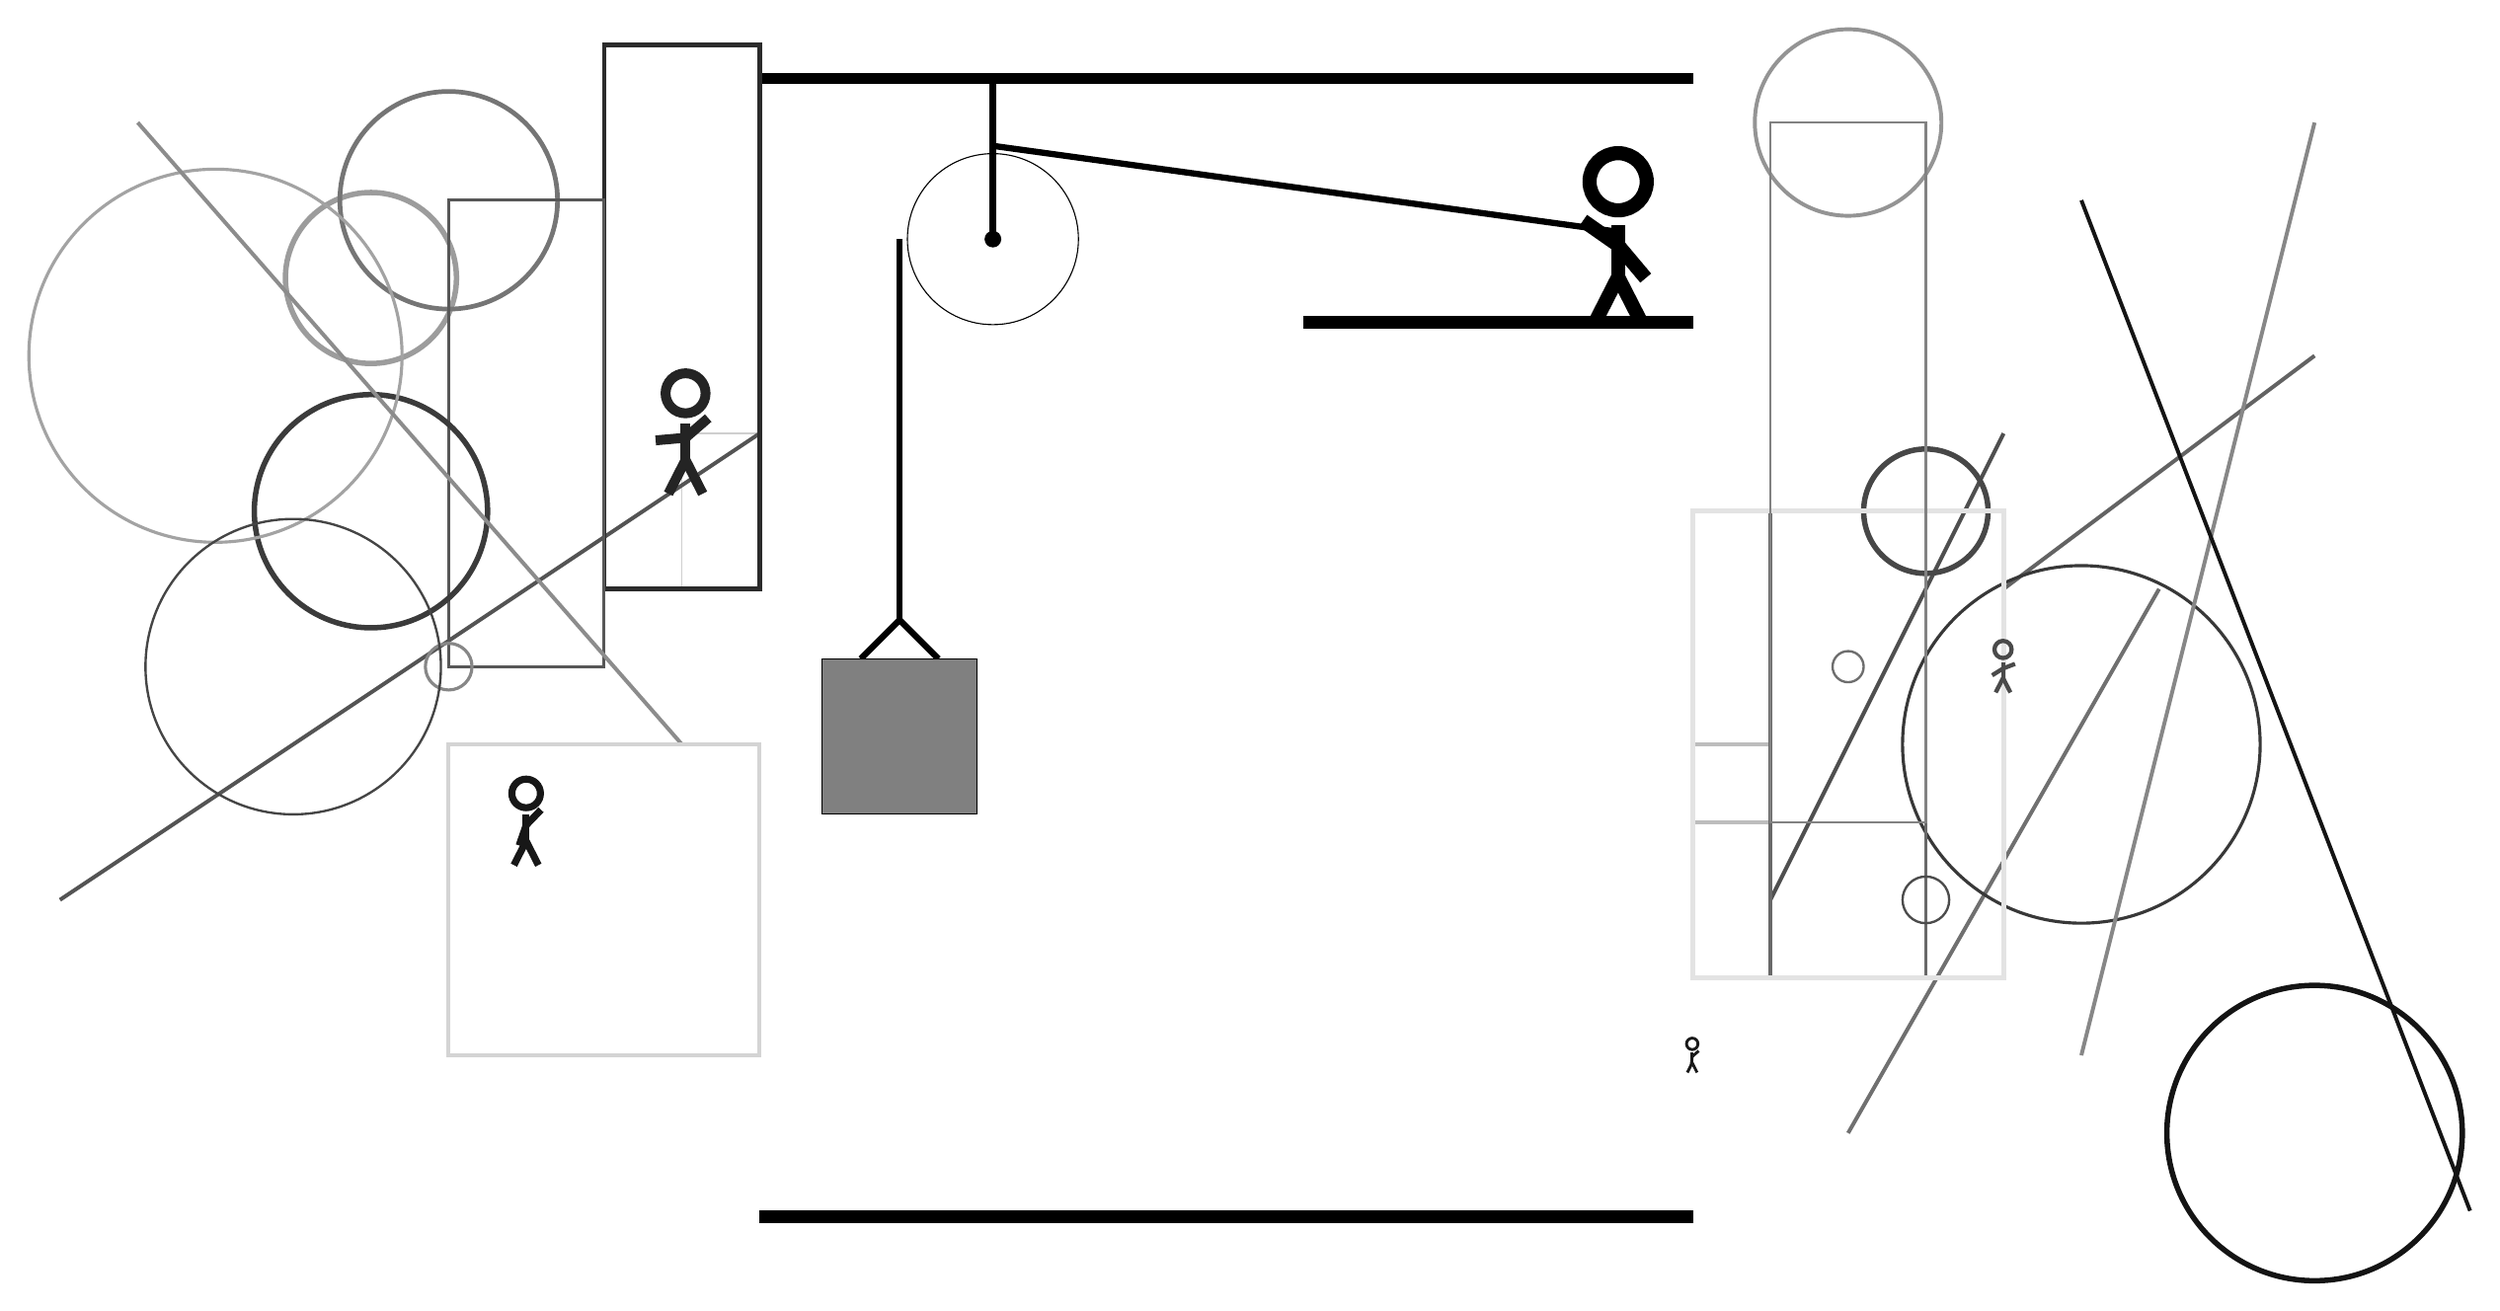
\begin{tikzpicture}
			%%%%% START %%%%%
			
			\draw[fill=black] (-2, 11.5) rectangle (10, 11.625);
			
			\draw[line width=0.5mm, color=black!69](14, 7) -- (11, 1);
			
			\draw[line width=0.2mm, color=black!19] (-3, 7) rectangle (-2, 5);
			\draw [line width=0.7mm, color=black!39](-7, 9) circle (1.1);
			\draw[line width=0.5mm, color=black!67](-2, 7) -- (-11, 1);
			\draw[line width=0.5mm, color=black!61](14, 5) -- (18, 8);
			\draw[line width=0.6mm, color=black!83] (-2, 5) rectangle (-4, 12);
			
			\draw [line width=0.6mm, color=black!54](-6, 10) circle (1.4);
			
			\draw[line width=0.4mm, color=black!66] (-4, 4) rectangle (-6, 10);
			\draw [line width=0.4mm, color=black!47](-6, 4) circle (0.3);
			
			\node[line width=0.4mm, color=black!86] at (-3, 7) {\Strichmaxerl[7][5][41]};
			\draw [line width=0.7mm, color=black!77](-7, 6) circle (1.5);
			\draw[line width=0.5mm, color=black!56](12, -2) -- (16, 5);
			\node[line width=0.2mm, color=black!90] at (10, -1) {\Strichmaxerl[2][83][41]};
			\draw [line width=0.4mm, color=black!78](15, 3) circle (2.3);
			\draw[line width=0.5mm, color=black!26] (11, 2) rectangle (10, 3);
			\node[line width=0.7mm, color=black!91] at (-5, 2) {\Strichmaxerl[5][71][46]};
			
			\draw [line width=0.5mm, color=black!42](12, 11) circle (1.2);
			
			\draw[line width=0.5mm, color=black!59] (11, 6) rectangle (13, 0);
			\draw [line width=0.4mm, color=black!36](-9, 8) circle (2.4);
			\draw [line width=0.7mm, color=black!72](13, 6) circle (0.8);
			\draw [line width=0.3mm, color=black!73](-8, 4) circle (1.9);
			
			\draw[line width=0.5mm, color=black!47](15, -1) -- (18, 11);
			\draw[line width=0.5mm, color=black!92](15, 10) -- (20, -3);
			\draw [line width=0.3mm, color=black!70](13, 1) circle (0.3);
			\draw[line width=0.5mm, color=black!45](-3, 3) -- (-10, 11);
			
			\draw[line width=0.6mm, color=black!11] (10, 0) rectangle (14, 6);
			
			\draw [line width=0.3mm, color=black!57](12, 4) circle (0.2);
			\node[line width=0.5mm, color=black!71] at (14, 4) {\Strichmaxerl[3][32][21]};
			\draw [line width=0.7mm, color=black!92](18, -2) circle (1.9);
			\draw[line width=0.3mm, color=black!49] (11, 11) rectangle (13, 2);
			\draw [line width=0.3mm, color=black!79](10, 6) circle (0.0);
			
			\draw[line width=0.5mm, color=black!17] (-2, -1) rectangle (-6, 3);
			
			\draw (1, 9.5) circle (1.1);
			\draw[fill=black] (1, 9.5) circle (0.1);
			\draw[line width=0.8mm] (1, 11.5) -- (1, 9.5);
			
			\draw[line width=0.8mm](-0.7, 4.1) --  (-0.2, 4.6) -- (0.3, 4.1);
			\draw[fill=black!50] (-1.2, 4.1) rectangle (0.8, 2.1);
			
			\draw[line width=0.8mm](-0.2, 9.5) -- (-0.2, 4.6);
			\centerarc[line width=0.8mm](1, 9.5)(90:180:1.2000000000000002)
			\draw[line width=0.8mm](1, 10.7) -- (9, 9.6);
			
			\node at (9, 9.5) {\Strichmaxerl[10][-35][-50]};
			\draw[fill=black] (5, 8.5) rectangle (10, 8.35);
			
			\draw[fill=black] (-2, -3) rectangle (10, -3.15);
			
			%%%%% END %%%%%
		\end{tikzpicture}
	\end{figure}	
\end{document}